\section{Developer Recommendation Preconditions}

Based on the results from these preliminary studies, we uncovered four concepts for making effective developer recommendations. At the minimum, these developer recommendation preconditions are required to make successful recommendations for software engineers. Below we define each of these concepts and provide examples with data collected from the completed evaluations, other software engineering research, and nudge theory literature:

\subsection{Demonstrate Desire}

In the \peer~study, we found that participants expressing  eagerness  to  use  a  recommended  tool led to more effective recommendations.  For example, during one study session a participant suggested using multi-level sorting functionality in Excel. Their partner, L11, demonstrated a desire to use the tool by  responding ``Oh!  Add  level!  Yes, awesome!" and adopted multi-level sorting for the remainder of the study tasks. This suggests recommending desirable tools and behaviors can increase adoption among developers. Meanwhile, in another case a participant asked their partner if they wanted to use the R statistical computing software\footnote{\url{https://www.r-project.org/}} to complete a task, but their partner responds ``No, no, no..." (S14). This shows how a lack of desire to use a specific tool can negatively impact the outcome of a recommendation. 

Software engineering research also suggests desire impacts the activities and behavior of developers. For example, Senyard and colleagues suggest that the desire of developers is important for motivating programmers to contribute to free and open source software and maintain successful projects~\cite{senyard2004have}. Furthermore, Murphy-Hill and colleagues found that one barrier to peer interactions is \textit{developer inertia}. This refers to when programmers do \textit{not} desire to share or learn about new software engineering tools because they ``feel that they do not need to discover a new tool because existing tools will do the job"~\cite[p.~16]{Murphy-Hill2015HowDoUsers}. These are examples of how the desire of software engineers can impact their behavior and decision-making when completing programming tasks.

Behavioral science research shows that humans often make poor decisions based on their desires. This is due to the fact that sometimes damaging behaviors provide short term benefits but have long term costs. Examples of these activities include smoking and eating junk food. Sunstein and Thaler argue humans need decision-making help in situations when ``choices and their consequences are separated in time...we get the pleasure now and suffer the consequences later...[these] are prime candidates for nudges"~\cite[p.~75]{sunstein2008nudge}. Nudges can be used to encourage the adoption of better behaviors by raising awareness of consequences for decisions. For example, nudges to teenagers in Montana were able decrease smoking rates among students by educating them on the dangers of smoking and providing information on the behaviors of peers~\cite{linkenbach2003most}. In some cases, poor developer behaviors may provide benefits to development teams. For example, Xiao and colleagues found that developers avoid adopting security tools that automatically check for vulnerabilities in code to save time and costs for training and implementing new systems~\cite{Xiao2014Security}. While avoiding useful developer behaviors may provide some benefits such as saving time and money, ignoring these practices can ultimately have serious consequences for development teams and their products over time. Nudges such as providing improved and more relevant feedback to users are an effective way to persuade developers to adopt better behaviors they may find undesirable by providing information and insight into the long term costs of avoiding these actions. 

\subsection{Familiarity}

Another key takeaway from the \peer~study is that users are more likely to adopt recommendations for tools and concepts they are familiar with it. In this study, we defined this criteria as users explicitly expressing familiarity with the environment surrounding a recommended tool. An example of an familiarity impacting the outcome of a recommendation in our experiment arose when L8 asked about using the \texttt{COUNTIF} function in Excel. L7 was familiar with the function and used the tool replying ``Yeah...here we go". However, we also found unfamiliarity negatively influenced adoption when a participant recommended using R to create a plot for analyzing the data, but their partner responded ``I don’t know R" (S9). In this case, the participant's unfamiliarity with R led to an ineffective recommendation. 

Familiarity can also lead to \textit{developer inertia}, where programmers prefer to stick with their familiar tools and workflow and avoid adopting better behaviors. Prior research also suggests familiarity can impact effectiveness and productivity at work. Goodman and colleagues found that the more knowledge employees have about the workplace and environment, or \textit{work familiarity}, improves performance~\cite{goodman1992familiarity}. Similarly in software engineering, Espinosa and colleagues found that familiarity impacts the completion of development tasks for distributed development teams~\cite{espinosa2002shared} while de Alwis and colleagues found that unfamiliarity in the Eclipse IDE made developers feel disoriented and negatively impacted productivity~\cite{de2006using}. For improving development tool adoption, Murphy-Hill and colleagues propose integrating familiarity into recommender systems by ranking commands based on similarity with collaborative filtering~\cite{Murphy-Hill2012Fluency}. Finally, Ko and colleagues suggest the majority of developers' time is spent learning about and becoming familiar with unfamiliar code, and code comprehension can impact other development activities and behaviors such as code navigation, searching, and tool usage~\cite{ko2006exploratory}. This indicates that familiarity plays a role in developer behavior and impacts their adoption of useful practices.

Research suggests humans are prone to make decisions based on previous experiences and rarely select options that are unfamiliar. Thaler and Sunstein note ``it is particularly hard for people to make good decisions when they have trouble translating the choices they face into the experiences they will have...when people have a hard time predicting how their choices will end up affecting their lives...a nudge might be welcomed"~\cite[p.~77-78]{sunstein2008nudge}. One example of an unfamiliar problem for many families face is selecting student loans. To account for unfamiliarity in student loan selections, Bettinger and colleagues implemented a nudge to incorporate the Free Application for Federal Student Aid (FAFSA) for student financial aid into the H&R Block\footnote{\url{https://www.hrblock.com}} tax return software, which many are more familiar with and utilize annually to complete their taxes. They found that this nudge made it easier to compare loan options and increased college enrollment among high school seniors~\cite{bettinger2013fafsa}. Many software engineers are comfortable with their current toolsets and environments, which leads to an unwillingness to try new useful development tools and processes. Nudges such as providing more information to software engineers when recommending unfamiliar development tools can help increase awareness and inform developers of new and better systems for completing programming tasks over their familiar methods.


\subsection{Social Context}

In the results from the \sorry~study, we found that one major issue with our \tele design is its lack of social context. Social context refers to the standard practices and activities necessary to participate in software engineering by interacting with developers and contributing to projects, specifically in open source software. In the \sorry~evaluation, many developers complained that \tool did not adhere to formatting guidelines when automatically adding the \EP plugin to project \textit{pom.xml} files. The most common social context complaint we received from GitHub users was that \tool messed up the whitespace of their project's maven \pom files when adding the \EP plugin (See Figure~\ref{fig:botse}b). One developer replied ``The automated tool you use messed up the pom.xml formatting to an extent that I could not see it" (P5). This suggests our bot's inability to adjust to the social context surrounding software development negatively impacted developers' likelihood to adopt recommendations.

Prior work also shows that social context is important in making recommendations to software engineers. Ahmadi goes as far as to argue that software engineering is a social activity~\cite{ahmadi2008survey}. To make effective recommendations, studies show it is important to integrate into this social context. For example, Wessel and colleagues evaluated the usage of bots in open source software and found that their inability to integrate into contributors' social context due to limited decision-making and poor feedback was the biggest challenge developers face interacting with bots and desired better interactions with users~\cite{wessel2018power}. Furthermore, prior work found that bots emulating humans receive better responses from developers and are more effective than recognizable bot accounts~\cite{murgia2016among}. Thus, effectively integrating recommendations with the social context of software engineering can impact developer adoption and perception of tools.

In \textit{Nudge}, the authors note ``one of the most effective ways to nudge (for good or evil) is via social influence"~\cite[p.~54]{sunstein2008nudge}. To study the impact of social nudges, Schultz and colleagues conducted a study that provided feedback to homeowners about the energy usage rates for their neighbors and households in a neighborhood in San Marcos, CA. They found that this nudge was able to drastically decrease usage and improve consumption decisions among users~\cite{schultz2007constructive}. Social recommendations are popular within software engineering. For example, badges are an effective way to present information about the status and condition of public projects, which can impact the behavior of contributors and other users~\cite{trockman2018badges}. In turn, we suggest nudges are an effective method to integrate recommendations for software engineers to adopt useful developer behaviors into the social environment of software engineering.

\subsection{Developer Workflow}

Another key result from \sorry was that the \tele in \tool disrupted the workflow of developers, or the processes required to complete programming tasks and deliver software. The most notable example of this was the fact that our automated pull requests for \EP often broke builds for repositories. Many projects have adopted continuous integration systems, such as TravisCI,\footnote{\url{https://travis-ci.org/}} to automatically build and integrate changes into projects. However, modifying projects to add a new static analysis tool often introduced many new errors and caused the build to fail. An example of this from our evaluation can be seen in Figure~\ref{fig:error}. Out of the 52 pull requests made, at least 17 resulted in a broken build. Many developers complained about this in their feedback on \tool, including P18 who commented ``This PR failed automatic checks, I think it should be closed". This interruption of developer workflow often discouraged users from merging pull requests from our system and accepting the recommendation.

Other work in software engineering also notes the importance of integration into the workflow of developers. For example, Sadowski found that one of the primary reasons developers at Google ignore static analysis tool warnings is because they are not integrated into their workflow~\cite{sadowski2018lessons}. Additionally, Viriyakattiyaporn and colleagues found that the inability to deliver suggestions within appropriate workflows discouraged programmers from following recommendations to improve code navigation with Spyglass~\cite{viriyakattiyaporn2009challenges} while Johnson and colleagues discovered that software engineers reported avoiding static analysis tools in their work due to a lack of customizability and poor integration into their existing processes~\cite{Johnson2013Why}. This points to a need to integrate recommendations to developer within their workflow to increase the adoption of useful behaviors to improve code quality and developer productivity. 

Nudges are useful for integrating recommendations into user workflows. For instance, a study conducted on Yale seniors found that a lecture on the risks of tetanus was ineffective (3\%) in convincing students to get a shot at the health center. However, providing a campus map to students with the health center circled in the same lecture convinced over nine times more people (28\%) to get the shot~\cite{leventhal1965specificity}. Even though the first group of students knew the location of the health center, nudges such as providing more details allowed students to know how to fit a visit into their weekly schedule and normal workflow. Software engineering research shows that integration into developer workflows is vital. To improve on the lack of tool adoption at Google, Sadowski implemented Tricorder to run numerous program analysis tools on code during code reviews~\cite{Tricorder}. Similarly, Balachandran found that integrating tools into the code review process with Review Bot at VMWare was able to reduce developer effort and improved code quality during code inspections~\cite{balachandran2013reducing}. These studies provide examples of how integration into developer workflow increased adoption of development tools. We believe this concept is key to improving the effectiveness of developer recommendations and encouraging adoption of useful developer behaviors.





% High spatial locality

% %\subsection{\timing}

% Location (hot and cold) [nudge theory] finds that timely feedback can improve acceptance of suggestion. Examples of these in real life? For example, handing out floss, right before entering a bathroom after eating ribs, increased chances of adopting flossing by 20\% (\todo{replace with example not completely made up}).

% To evaluate the timing of digital nudges, we introduce the concept of \emph{just-in-time nudges}. These nudges make recommendations to developers at a moment when a software engineering behavior is appropriate.

% We hypothesize that developers will prefer just-in-time nudges when a software engineering tool is most applicable over nudges presented at different times. Recommendations made when they are appropriate provide more convenience to users so developers don't have to figure out when's the best time to use a tool or practice. This can help improve adoption of software engineering behaviors for developers while they are completing programming tasks. A potential downside to just-in-time nudges is that they can interrupt developers in their work, which research suggests may lead to a loss of task context~\cite{parnin2010interrupted}.

% High temporal locality

\begin{figure*}
\centering
	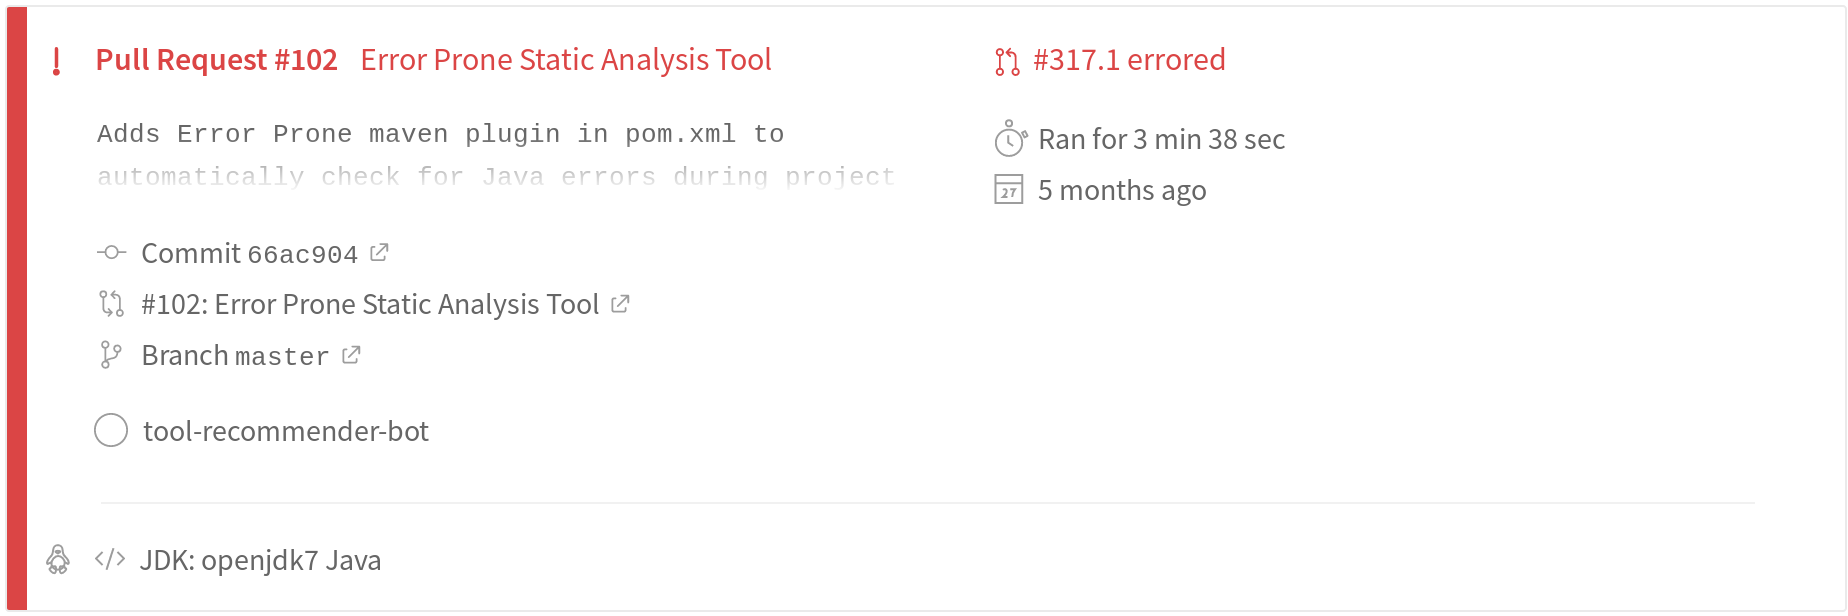
\includegraphics[width=\textwidth]{images/error.png}
	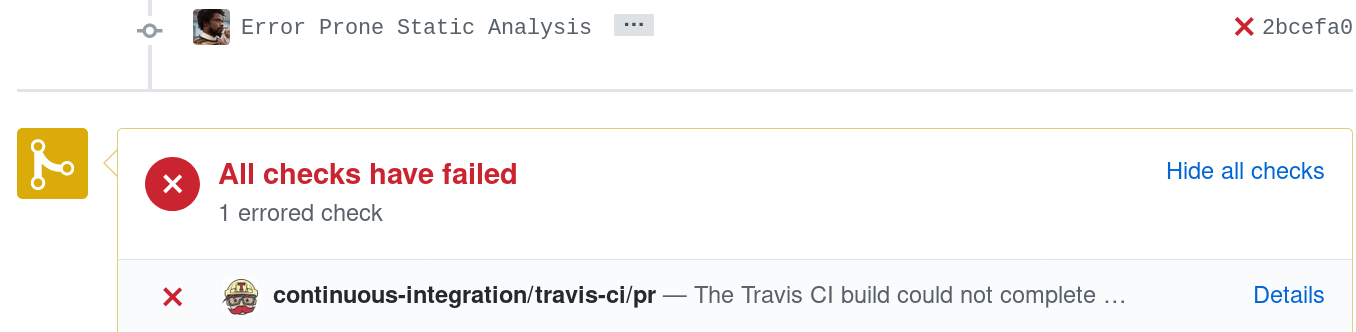
\includegraphics[width=\textwidth]{images/error2.png}
	\caption{Examples of automated pull requests from \tool causing projects' continuous integration builds to fail}	
	\label{fig:error} 
\end{figure*}


% %\subsection{Public nudge}

% %Humans are more likely to adopt behavior if there is external pressure to do so.

% %We define \textit{public nudges} as nudges that are visible and available to see by a specific community. They may also involve social pressure if certain behaviors aren't adopted. For example, badges on GitHub are public nudges viewable to users who visit a repository and can influence their decision to contribute or use the product. These badges display whether projects adopt certain software engineering behaviors, such as passing builds. Figure \ref{fig:red_badge} presents a badge for a project that does not use a useful software engineering processes during development, while the developers for a project with a badge in Figure \ref{fig:green_badge} integrate software engineering behaviors in their development process. Trockman and colleagues examined the effect of these public nudges for npm\footnote{https://www.npmjs.com/} packages on GitHub and found that the addition of badges correlated with improvements in the quality of the project, i.e. adding a quality assurance badge displaying code coverage increased the coverage of tests~\cite{trockman2018badges}

% %Our hypothesis is that developers are more likely to adopt useful software engineering behaviors if they are publicly nudged to do so.

% % \begin{figure}
% % \centering
% % \subfigure[Project without a software engineering behavior]{
% % \label{fig:red_badge}
% % 
\includegraphics[width=\textwidth/2]{images/badge1.png}}
% % \qquad
% % \subfigure[Project with a software engineering behavior]{
% % \label{fig:green_badge}
% % 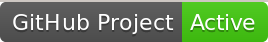
\includegraphics[width=\textwidth/2]{images/badge2.png}}
% % \caption{Example of a public nudge}
% % \end{figure}

% % [benefits/trade-offs;hypothesis]

% % \subsection{Social nudge}

% % Nudge theory finds that people are more likely to adopt a useful behavior if others they know already do it. Perloff studied the impact of social media on body image and self-perception among American girls, and proposes using ``media-based interventions...to nudge individuals into changing their attitudes and behaviors"~\cite[p.~364]{perloff2014social}. This work suggests social media use is key in creating social comparisons and influencing users to adopt harmful behaviors such as body dissatisfaction and eating disorders.

% % To study digital nudges in a social context, we introduce \textit{social nudges}. These nudges suggest software engineering behaviors that have been adopted by a developer's friends or colleagues. An example of this is seen in prior work examining peer interactions. Murphy-Hill conducted interviews and surveys with software engineers and found that developers prefer recommendations from peers over other methods of tool discovery such as tutorials, discussion threads, tool encounters, and written descriptions~\cite{Murphy-Hill2015HowDoUsers}.

% % Our hypothesis is that developers are more likely to adopt behaviors recommended in a nudge if they know it is used by a friend or colleague.

% % \subsection{Apprehensive nudge}

% % If you can show a target behaviors usefulness by presenting multiple places it can be applied, people are more likely to adopt it.

% % We created the concept of \textit{apprehensive nudges}, which provide multiple locations where software engineering activities can be applied, to study how this impacts activity adoption for developers.


% % \subsection{Automated nudge}

% % If you do the work for them, humans are more likely to adopt specific behaviors. \todo{Example= automatic magazine subscription renewal due to status quo bias [Nudge, 35]}

% % To determine if automatically performing software engineering behaviors for developers impacts adoption for developers, we introduce \textit{automated nudges}. There are many ways automation is used to improve software engineering and help developers adopt helpful behaviors. For instance, Mirhosseini and colleagues investigated creating automated pull requests to convince developers to upgrade outdated dependencies using greenkeeper\footnote{https://greenkeeper.io} to manage dependency package versions for GitHub projects~\cite{sam2017autopullrequests}. They found that automated pull requests were useful in increasing awareness of out-of-date package dependencies to developers.

% % [benefits/trade-offs;hypothesis]

% % \subsection{Tutorial nudge}

% % If you show people how to do a certain behavior, then they are more likely to adopt it.

% % We define \textit{tutorial nudges} as digital nudges that show developers how to use a specific software engineering tool or programming activity. For example,...

% % [Conceptual implementation]

% % [benefits/trade-offs;hypothesis]

% % \subsection{Reminder nudge}

% % If you continually remind humans to adopt a certain activity, they are more likely to adopt it.

% % To evaluate the effectiveness of reminders, we developed \textit{reminder nudges} to periodically recommend useful software engineering behaviors to programmers.

% % [Conceptual implementation]

% % [benefits/trade-offs;hypothesis]

% % \subsection{Positive nudge}

% % Nudge theory suggests using positive language is more effective in helping people adopt target behaviors. For example, Doberstein and colleagues evaluated using positive messages to improve attitudes about increasing residential housing density in Canada~\cite{doberstein2016positive}. They compared a neutral control statement of benefits with public statements, private statements, and expert comparisons.  \todo{Framing [Nudge, 36-37]}

% % To determine if developers respond better to positive or negative recommendations, we introduce \textit{positive nudges} that commend developers for their work rather than blaming them to encourage future software engineering behavior adoption.

% % \subsection{Effects}

% % We hope our nudges have some of the following effects on developers who receive recommendations for software engineering behaviors...

% % \todo{Some interesting effects to consider:}
% % \begin{itemize}
% % \item Baader-Meinhof --- you start seeing something you just learned or on your mind everywhere.
% % \item Diderot Effect --- the act of getting one new thing triggers a cascade of other new things.
% % \item Novelty Effect --- using something new makes you think you are more productivity
% % \item ... should look at behavioral and marketing psychology stuff...
% % \end{itemize}
